\section{Introduction} \label{sec:introduction}
% Vision

There is a growing interest in deploying autonomous systems in unstructured environments to perform complex manipulation tasks for different applications like assistive service in the healthcare domain~\cite{cooper2020ari}, agrifoods~\cite{duckett2018agricultural}, and industrial inspection and maintenance~\cite{lattanzi2017review}. Mobile manipulator robots present a compelling choice to tackle these problems since they combine an unconstrained workspace with highly dexterous interaction capabilities. However, to fully exploit these capabilities, systems require planning and control algorithms that can generate fast, accurate, and coordinated reactive whole-body motions that account for multiple potential contacts with the environment. 

% Motivation
\subsection{Problem Statement}


In this work, we focus on whole-body coordination and manipulation of articulated objects, e.g., to open drawers or doors (see \fig\ref{fig:royal_panda}). 
These tasks involve a high degree of physical interaction, which necessitates a stable control strategy that is able to exploit contacts to successfully manipulate the articulated object while satisfying joint and input constraints.

\subsection{Related Works}

% Existing methods
While traditional ``plan-and-act'' frameworks break down such tasks into subproblems that are easier to solve (e.g. reach, grasp, pull)~\cite{Murali2020}, they do not offer fast and control-aware replanning, which is crucial for mobile manipulation operations in dynamic and uncertain environments. We observe that humans heavily rely on their physical understanding of the surrounding environment and thus we believe that a robot needs to consider this aspect as well when planning for the optimal actions.

With the recent advancements in artificial intelligence, reinforcement learning (RL) is a promising method to solve a range of robotic control tasks, including manipulation~\cite{finn2016deep}, as they learn an end-to-end representation of the optimal policy. However, real-world applications of RL typically require training times that are not practical for physical hardware and suffer from the well-known \textit{sim-to-real} gap~\cite{chebotar2019closing}. 
On the other side of the spectrum, Model Predictive Control (MPC) has gained broad interest in the robotics community thanks to its capability of dealing with input constraints and task objectives by solving a multivariate optimization problem or using the \textit{principle of optimality}. 
MPC has been successfully applied to aerial robots~\cite{brunner2020trajectory}, autonomous racing~\cite{liniger2015optimization}, legged locomotion~\cite{grandia2019frequency}, and whole-body control~\cite{minniti2019whole}. 
Nevertheless, MPC requires a model that is locally differentiable with respect to the input and the state~\cite{buchli2017optimal}. On the other hand, manipulation tasks involve changes in the contact state causing sharp discontinuities in both the cost and system dynamics, thus directly violating the differentiability requirements. 


\begin{figure}[t]
\centering
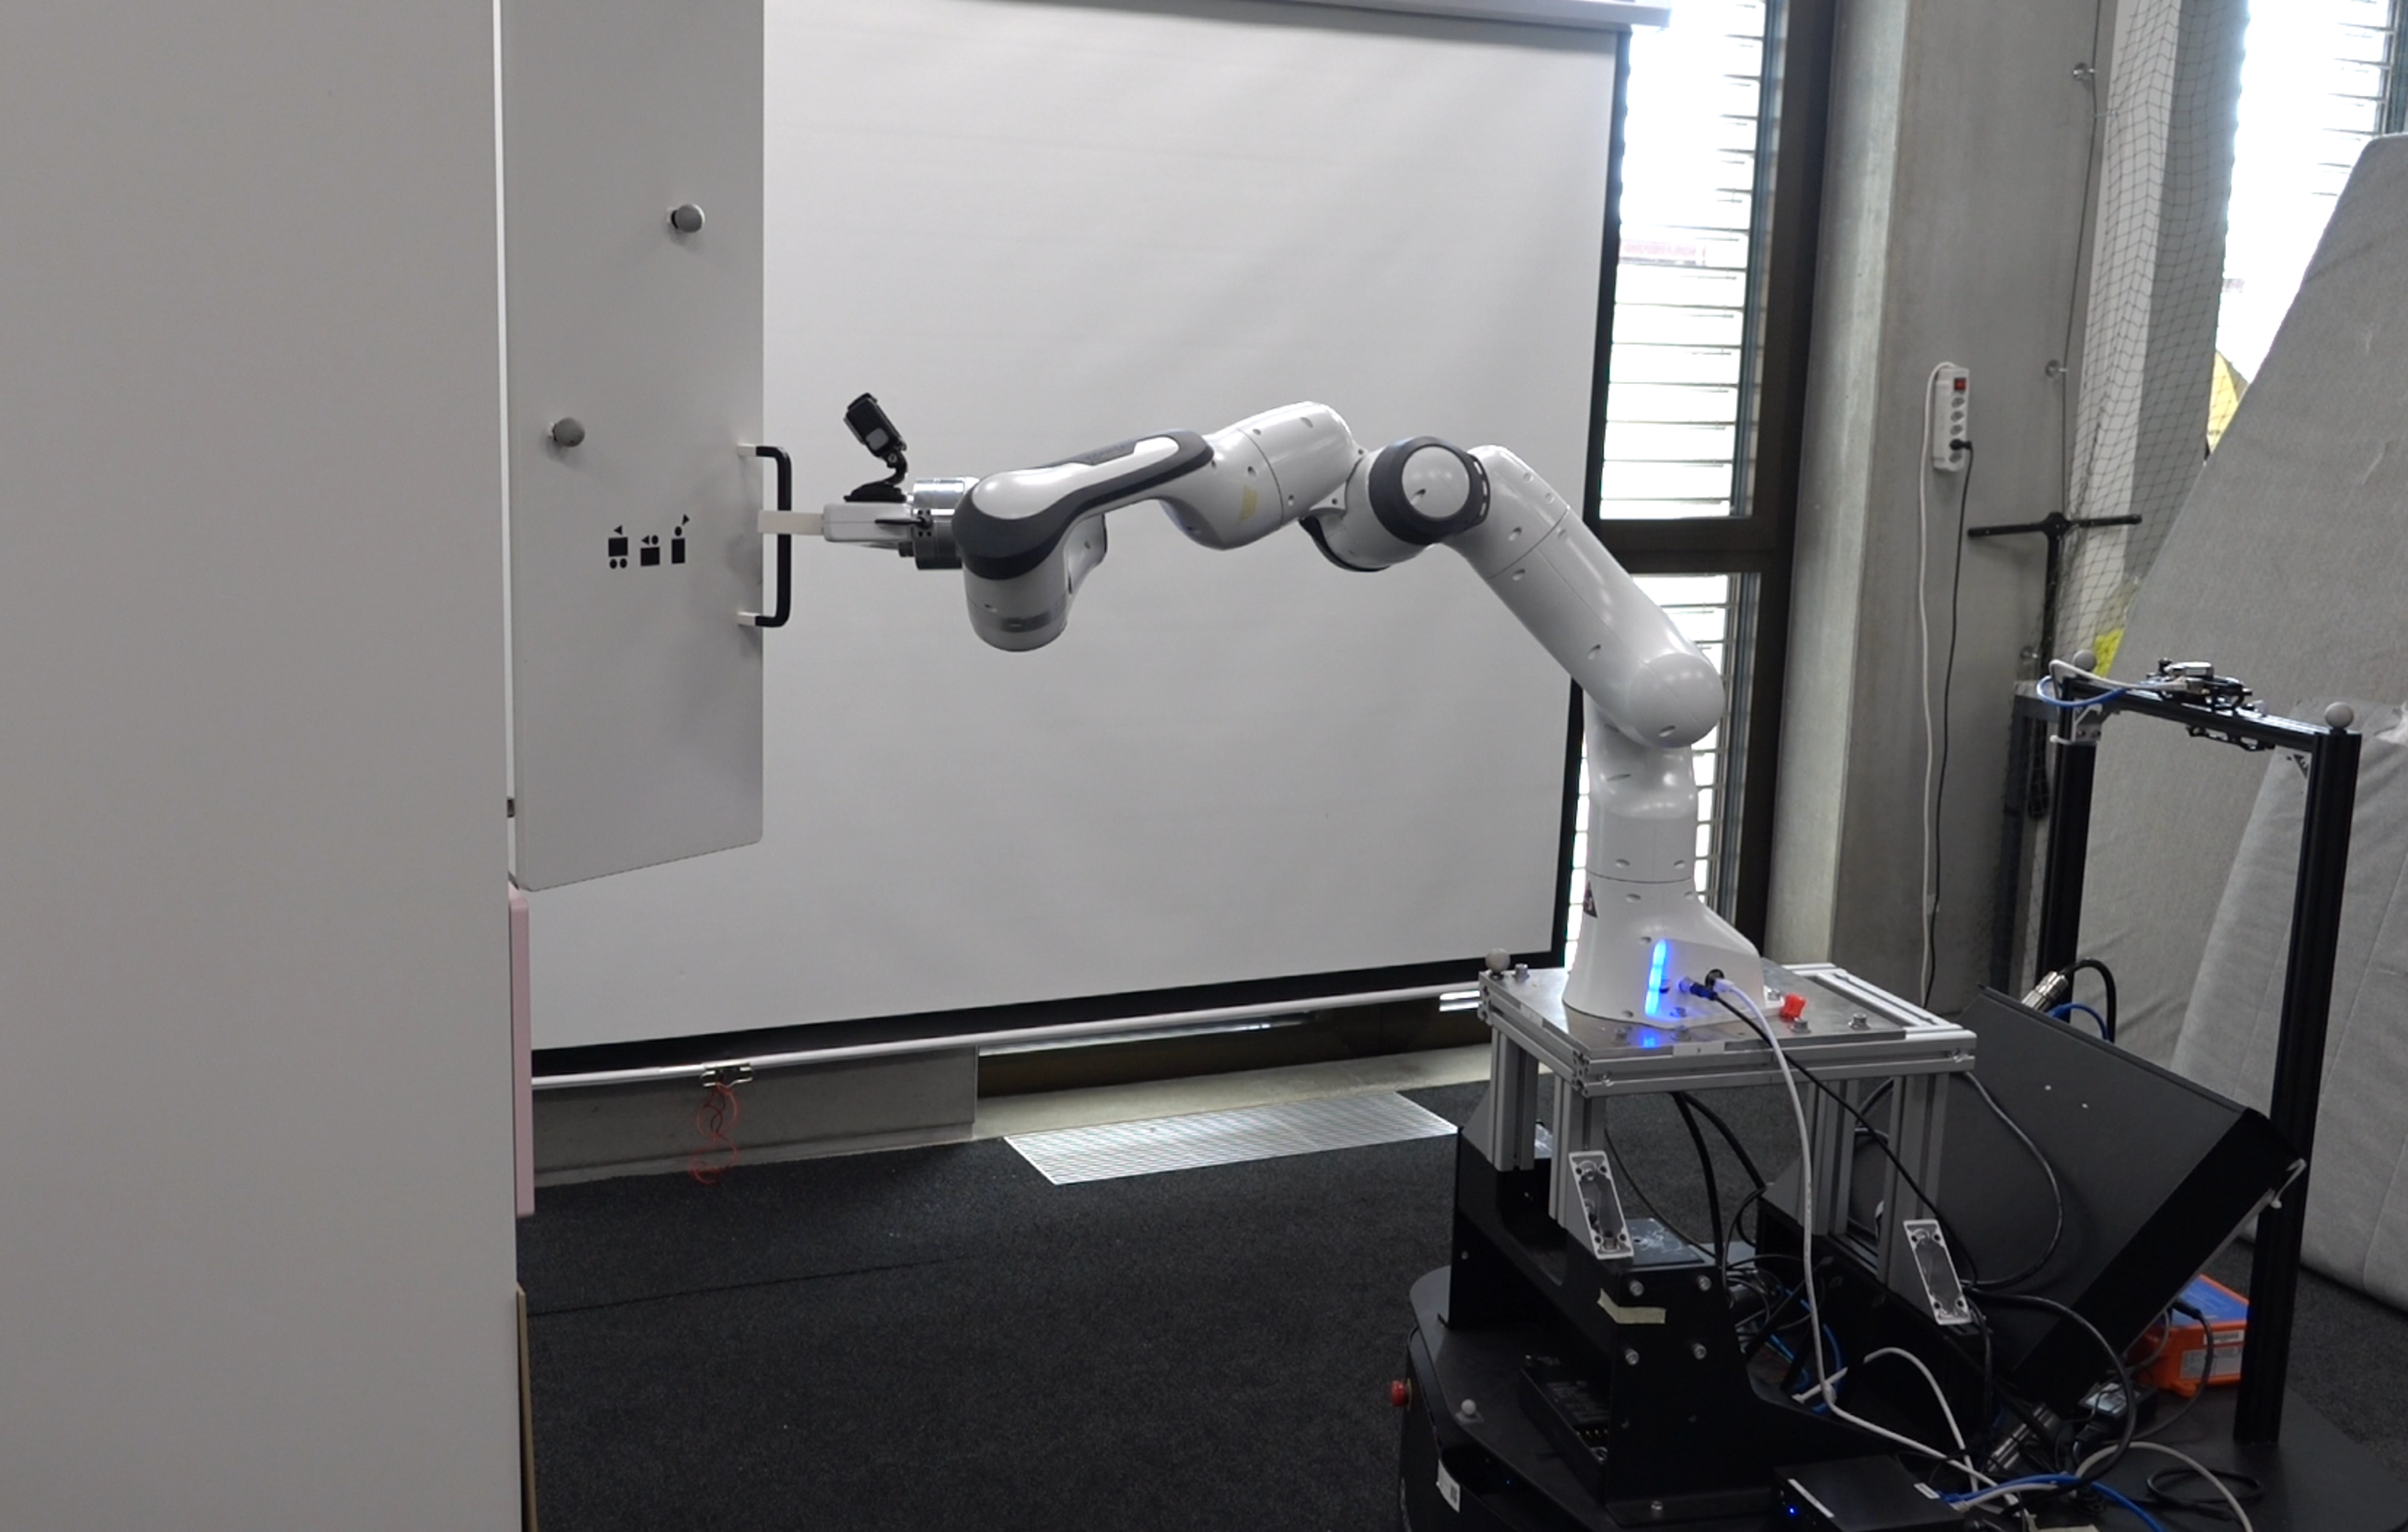
\includegraphics[trim={0 0 0 100},clip,width=0.9\columnwidth]{framework_manipulation/figures/hardware/system_figure.pdf}
\caption{\textit{RoyalPanda}, a 10-DOF mobile manipulator while performing a door opening task.} \label{fig:royal_panda}
\end{figure}

% Performance : sampling control
Recently, sampling-based methods have emerged and advanced in theory and applications~\cite{lee_aggressive_2020,abraham_model-based_2020,williams_information_nodate,williams_information_2017,rajamaki_augmenting_2017}. 
In contrast to traditional MPC, sampling methods stem from a probabilistic interpretation of the control problem. 
Rather than solving a complex optimization problem, they rely on sampling system trajectories, referred to as \textit{rollouts}, and ``weighting'' them according to the cumulative cost so that only favorable trajectories survive the iterative sampling process. The only requirement is that it is possible to forward simulate the system evolution. This has been exploited to control camera motions for target tracking in drone racing~\cite{lee_aggressive_2020}, robot arm motions for manipulation tasks~\cite{abraham_model-based_2020}, and for generating aggressive driving maneuvers such as drifting~\cite{williams_information_nodate, williams_information_2017}. 

% Gap 
Yet despite their appealing features, sampling-based methods can be costly to execute and solution quality is highly dependent on sampling quality. Previous works argue that thousands of trajectories need to be sampled in real time for the effectiveness of the proposed sampling-based algorithm and therefore GPU-based simulation is needed for fast parallel computation~\cite{williams_model_2017}. 
Unfortunately, GPUs are not common on mobile robots (e.g., because of limited power and payload) and often the overall computation times are still not adequate for feedback control. 
Furthermore, demonstrations on real systems involving different physical interactions (e.g. a robot arm opening a drawer~\cite{abraham_model-based_2020}) have typically only been shown by breaking down the multi-contact task into stages and enforcing constraints when switching between them. 
This can limit the control envelope of the system and sacrifices solution optimality. For example, it is common practice to fix the gripper orientation between successive reach and pull stages and perform manipulation under a rigid grasp. In the presence of uncertainty and tracking errors, this often leads to high contact forces and dangerous behaviors.

% Safety : Barrier functions
In fact, a dual aspect of performance is safety. Safety-critical constraints are only integrated through additional cost terms, penalizing unsafe paths but not prohibiting them. As a consequence, constraints fulfillment merely relies on sampling of "safe" trajectories. 
Recently \emph{Control Barrier Functions} (CBFs) have been introduced as a mean to constrain the system to a safe set. The safe set defines the locus where all safety requirements are met, e.g. no self-collision happens and joint limits are fulfilled. CBFs are expressed as affine inequality constraints in the control input that satisfied point-wise in the candidate safe set, imply forward invariance of the set, hence safety \cite{ames2016control}.  Often a controller is implemented by joining a \emph{Control Lyapunov Functions} and a \emph{Control Barrier Function} in a unique optimization problem, where the latter is treated as a hard constraint. This control method has been successfully deployed in safety-critical applications such as Adaptive Cruise Control and Lane Keeping \cite{vahidi2003research}, segway stabilization \cite{gurriet2018towards} and collaborative robotics \cite{benzi2021optimization}.

% Stability : passivity
Last but not least, these methods do not provide any stability and safety guarantees which, especially during autonomous interaction, are as important as performance. In this context, we are interested in a stable interaction with an \emph{a priori} poorly known environment. This lack of knowledge might come from sensing limitations or a model mismatch. Passivity analysis has drawn attention in recent years, as a way to analyze the stability of a controlled system. Intuitively, a passive system cannot produce more energy than what is stored in it. The question that arises is then how to design a controller which makes the system passive at all time. A rather new approach, is to use an auxiliary virtual system called \emph{energy tank} as a storing element containing a bounded amount on energy, or energy budget, to perform the task. Boundness ensures passivity \cite{secchi2019energy} and therefore a robust behavior during interaction. Energy tanks have been deployed in many robotics applications such as for impedance controllers with time-varying stiffness \cite{schindlbeck2015unified}, force-impedance control \cite{shahriari2018valve}, and lately with CBFs for controlling a robotic arm \cite{benzi2021optimization}.

\subsection{Contributions}

We propose a practical and robust receding horizon algorithm that achieves real-time whole-body control of a mobile manipulator using only a laptop CPU. Our work is based on an iterative sampling of control trajectories. Safety and stability are ensured through a sequential optimization problem that finds the closest policy to the optimized one, which enforces constraints and passivity of the autonomous system. g

Our main contribution is a new framework for mobile manipulation which combines tools from stochastic optimization, safety-critical control, and passivity theory.

% Results
To demonstrate the applicability and effectiveness of this approach, we perform several ablation studies in simulation on kinematic and dynamical manipulators and deploy the full algorithm on our \textit{RoyalPanda} platform (a 7-DOF Franka Emika Panda arm mounted on the holonomic Clearpath Ridgeback base, \fig\ref{fig:royal_panda}) for a target reaching and door opening task. An open source implementation of our solution is provided at \url{https://git.io/Jtda7}.

In summary, the contributions of the present work are as follows:
\begin{enumerate}
    \item A framework for safe interaction-aware receding horizon control of a mobile manipulator,
    \item practical insights and a new power-aware cost formulation focused on mobile manipulation tasks,
    \item an experimental evaluation of the effectiveness of the approach and of the contribution of each algorithmic component,
    \item hardware experiments showing the applicability of the approach for real-time operation,
    \item an open source implementation of the proposed method including a multi-threaded sampling based controller and an efficient quadratic program for addressing kinematic and dynamic constraints.
    \end{enumerate}

\subsection{Overview}

The remainder of the paper is organized as follows. In 
\sect \ref{sec:formulation} the manipulation problem is fist formulated. In \sect \ref{sec:theory} we review the main theoretical background introducing receding horizon sampling-based control, the concept of barrier function and energy tanks. In the following \sect \ref{sec:control_method} these tools are combined in a unified control method focusing on performance and safety. We evaluate the overall framework in \sect \ref{sec:experiments} and conclude with  hardware experiments which to show its applicability to the real platform. 
